\subsection{UC5: Gestione degli alert}
\begin{figure} [H]
 	\centering
 	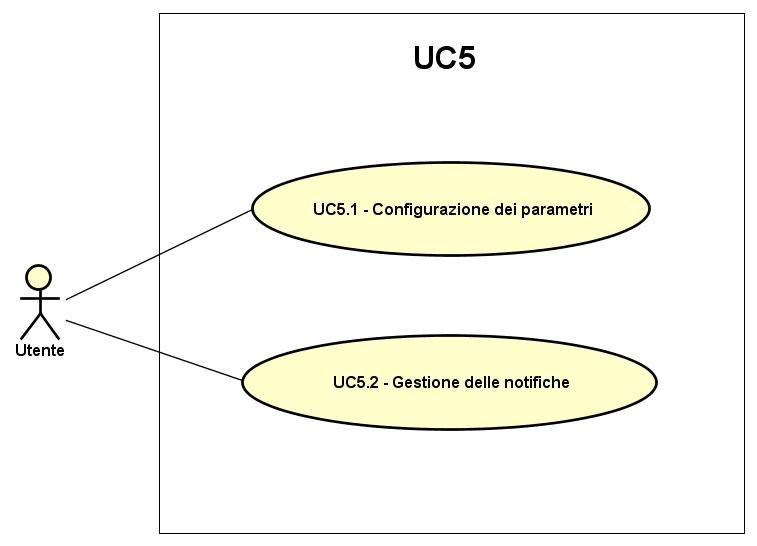
\includegraphics[scale=0.45]{Img/UC5}
 	\caption{UC5: Gestione degli alert}\label{}
\end{figure}
\begin{itemize}
	\item \textbf{Attori}: Utente;
	\item \textbf{Descrizione}: L'attore configura le opzioni relative ad \gl{alert} personalizzati;
	\item \textbf{Precondizione}: Il \gl{plugin} deve leggere un flusso di dati;
	\item \textbf{Flusso principale degli eventi}:
		\begin{itemize}
			\item Configurazione dei parametri (UC5.1);
			\item Gestione delle notifiche (UC5.2).
		\end{itemize}
	\item \textbf{Postcondizione}: Gli alert e le notifiche di attivazione sono stati configurati.
\end{itemize}

\subsection{UC5.1: Configurazione dei parametri}
\begin{figure} [H]
	\centering
	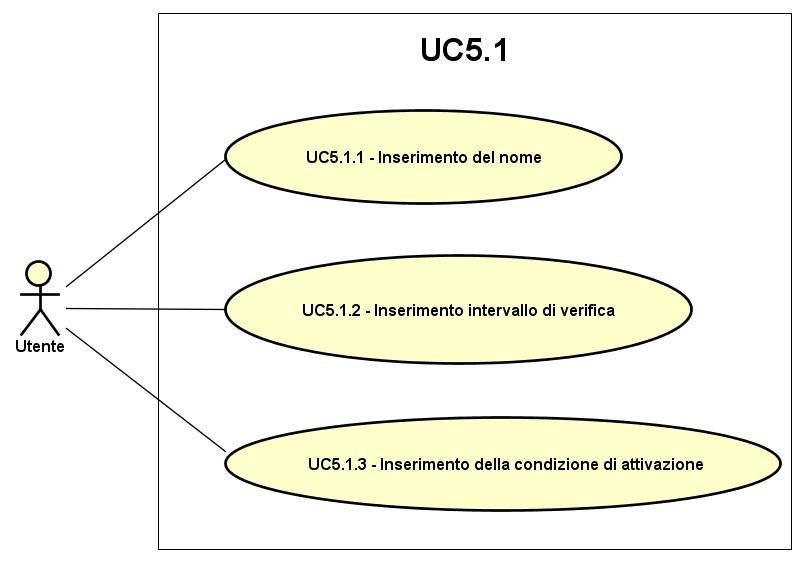
\includegraphics[scale=0.45]{Img/UC5-1}
	\caption{UC5.1: Configurazione dei parametri}\label{}
\end{figure}
\begin{itemize}
	\item \textbf{Attori}: Utente;
	\item \textbf{Descrizione}: L'attore configura i parametri che definiscono un alert;
	\item \textbf{Precondizione}: Il sistema permette la configurazione dei parametri di un alert;
	\item \textbf{Flusso principale degli eventi}:
		\begin{itemize}
			\item Inserimento del nome (UC5.1.1);
			\item Inserimento intervallo di notifica (UC5.1.2);
			\item Inserimento della condizione di attivazione (UC5.1.3).
		\end{itemize}
	\item \textbf{Postcondizione}: L'alert è stato configurato.
\end{itemize}

\subsection{UC5.1.1: Inserimento del nome}
\begin{itemize}
	\item \textbf{Attori}: Utente;
	\item \textbf{Descrizione}: L'attore inserisce il nome dell'alert;
	\item \textbf{Precondizione}: Il sistema permette l'inserimento del nome di un alert;
	\item \textbf{Postcondizione}: Il nome dell'alert è stato inserito.
\end{itemize}

\subsection{UC5.1.2: Inserimento intervallo di verifica}
\begin{itemize}
	\item \textbf{Attori}: Utente;
	\item \textbf{Descrizione}: L'attore inserisce l'intervallo di verifica ed una eventuale durata minima della condizione di attivazione per notificare l'alert;
	\item \textbf{Precondizione}: Il sistema permetta l'inserimento dell'intervallo di verifica di un alert;
	\item \textbf{Postcondizione}: L'intervallo di verifica dell'alert è stato inserito.
\end{itemize}

\subsection{UC5.1.3: Inserimento della condizione di attivazione}
\begin{itemize}
	\item \textbf{Attori}: Utente;
	\item \textbf{Descrizione}: L'attore inserisce la condizione necessaria per l'attivazione dell'alert;
	\item \textbf{Precondizione}: Il sistema permette l'inserimento di una condizione di attivazione di un alert;
	\item \textbf{Postcondizione}: La condizione di attivazione dell'alert è stata inserita.
\end{itemize}

\subsection{UC5.2: Gestione delle notifiche}
\begin{itemize}
	\item \textbf{Attori}: Utente;
	\item \textbf{Descrizione}: L'attore seleziona il modo in cui viene notificata l'attivazione di un alert;
	\item \textbf{Precondizione}: Il sistema permette di notificare l'attivazione di un alert;
	\item \textbf{Postcondizione}: Il modo in cui viene notificata l'attivazione di un alert è stato selezionato.
\end{itemize}

\subsection{UC8: Pubblicazione snapshot}
\begin{figure} [H]
	\centering
	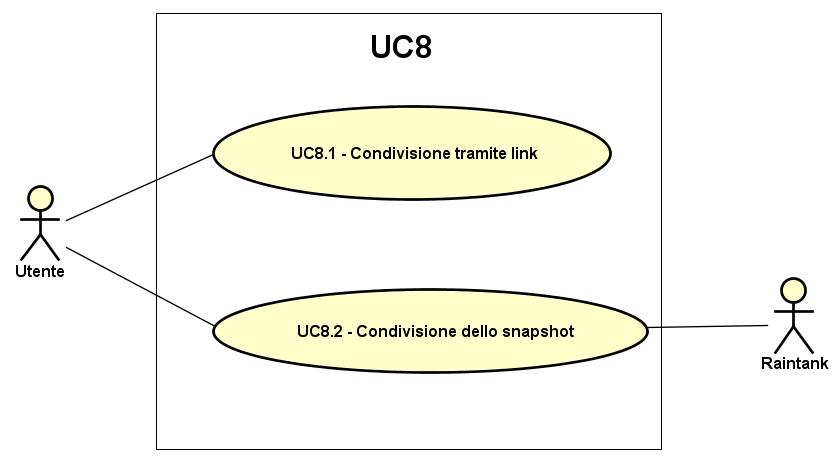
\includegraphics[scale=0.45]{Img/UC8}
	\caption{UC8: Pubblicazione snapshot}\label{}
\end{figure}
\begin{itemize}
	\item \textbf{Attori}: Utente;
	\item \textbf{Descrizione}: L'attore può salvare lo \gl{snapshot} della dashboard o di un panel;
	\item \textbf{Precondizione}: Il sistema permette il salvataggio di snapshot;
	\item \textbf{Flusso principale degli eventi}:
	\begin{itemize}
		\item Pubblicazione su istanza (UC8.1);
		\item Pubblicazione su Raintank (UC8.2);
		\item Configurazione opzioni di pubblicazione (UC8.3).
	\end{itemize}
	\item \textbf{Postcondizione}: Lo snapshot è stato salvato.
\end{itemize}

\subsection{UC8.1: Pubblicazione su istanza locale}
\begin{itemize}
	\item \textbf{Attori}: Utente;
	\item \textbf{Descrizione}: L'attore pubblica lo snapshot della dashboard o di un panel sulla sua istanza locale;
	\item \textbf{Precondizione}: Il sistema permette la pubblicazione di snapshot sull'istanza di un utente;
	\item \textbf{Postcondizione}: Lo snapshot è stato pubblicato sull'istanza.
\end{itemize}

\subsection{UC8.2: Pubblicazione su Raintank}
\begin{itemize}
	\item \textbf{Attori}: Utente;
	\item \textbf{Descrizione}: L'attore pubblica lo snapshot della dashboard o di un panel sulla piattaforma \gl{Raintank};
	\item \textbf{Precondizione}: Il sistema permette la pubblicazione di snapshot su Raintank;
	\item \textbf{Postcondizione}: Lo snapshot è stato pubblicato su Raintank.
\end{itemize}

\subsection{UC8.3: Configurazione opzioni di pubblicazione}
\begin{figure} [H]
	\centering
	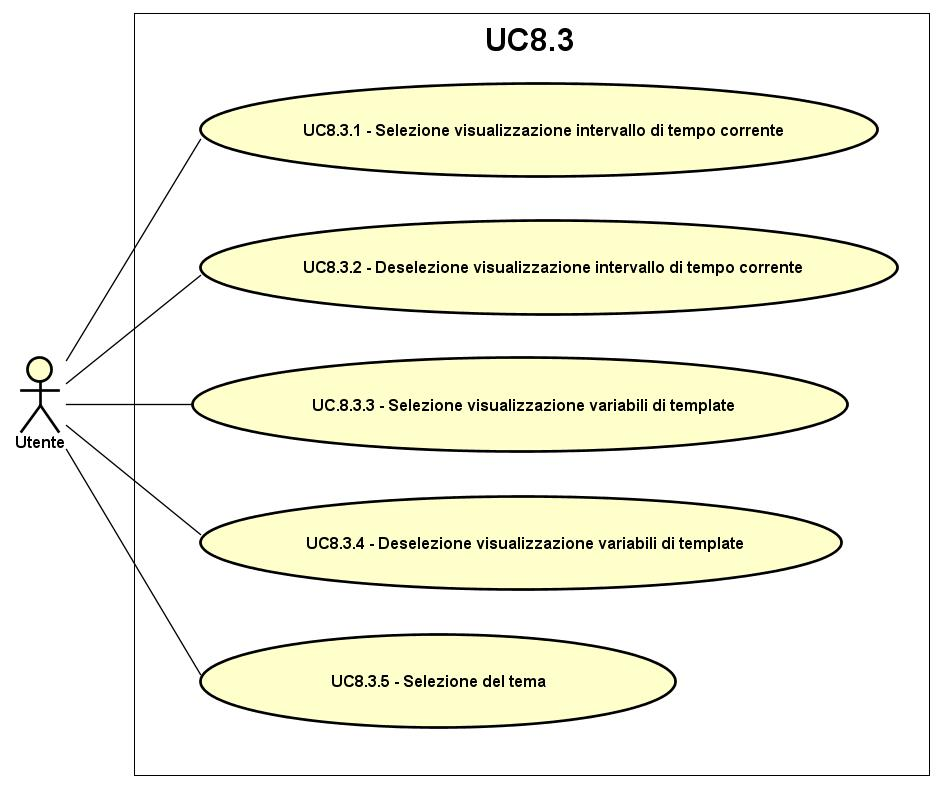
\includegraphics[scale=0.45]{Img/UC8-3}
	\caption{UC8.3: Configurazione opzioni di pubblicazione}\label{}
\end{figure}
\begin{itemize}
	\item \textbf{Attori}: Utente;
	\item \textbf{Descrizione}: L'attore configura le opzioni per la pubblicazione dello snapshot della dashboard o di un panel;
	\item \textbf{Precondizione}: Il sistema permette di configurare le opzioni per la pubblicazione di snapshot;
	\item \textbf{Flusso principale degli eventi}:
		\begin{itemize}
		\item Inserimento del nome (UC8.3.1);
		\item Selezione tempo di permanenza (UC8.3.2);
		\item Inserimento tempo per timeout (UC8.3.3).
	\end{itemize}
	\item \textbf{Postcondizione}: Le opzioni per la pubblicazione dello snapshot sono state configurate.
\end{itemize}

\subsection{UC8.3.1: Inserimento del nome}
\begin{itemize}
	\item \textbf{Attori}: Utente;
	\item \textbf{Descrizione}: L'attore inserisce il nome dello snapshot;
	\item \textbf{Precondizione}: Il sistema permette l'inserimento del nome di uno snapshot;
	\item \textbf{Postcondizione}: Il nome dello snapshot è stato inserito.
\end{itemize}

\subsection{UC8.3.2: Selezione tempo di permanenza}
\begin{itemize}
	\item \textbf{Attori}: Utente;
	\item \textbf{Descrizione}: L'attore seleziona il tempo di permanenza di uno snapshot dal momento della sua pubblicazione;
	\item \textbf{Precondizione}: Il sistema permette di selezionare il tempo di permanenza di uno snapshot tra le opzioni predefinite;
	\item \textbf{Postcondizione}: Il tempo di permanenza dello snapshot è stato selezionato.
\end{itemize}

\subsection{UC8.3.3: Inserimento tempo di timeout}
\begin{itemize}
	\item \textbf{Attori}: Utente;
	\item \textbf{Descrizione}: L'attore inserisce il tempo(in secondi) massimo per il caricamento dei dati nello snapshot;
	\item \textbf{Precondizione}: Il sistema permette l'inserimento del tempo massimo per il caricamento dei dati di uno snapshot;
	\item \textbf{Postcondizione}: Il tempo di timeout è stato inserito.
\end{itemize}

\subsection{UC9: Condivisione snapshot}
\begin{figure} [H]
	\centering
	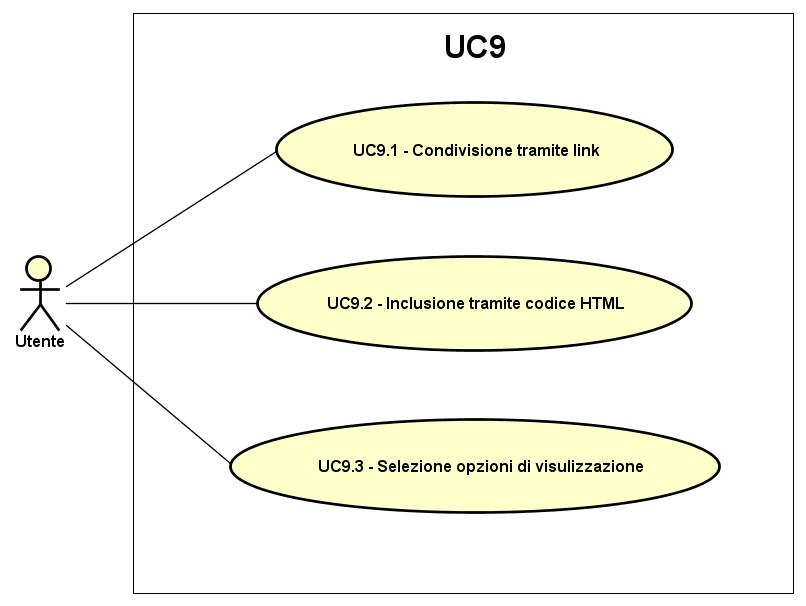
\includegraphics[scale=0.45]{Img/UC9}
	\caption{UC9: Condivisione snapshot}\label{}
\end{figure}
\begin{itemize}
	\item \textbf{Attori}: Utente;
	\item \textbf{Descrizione}: L'attore condivide lo snapshot della dashboard o di un panel e ne configura le opzioni di visualizzazione;
	\item \textbf{Precondizione}: Il sistema permette la condivisione di snapshot;
	\item \textbf{Flusso principale degli eventi}:
	\begin{itemize}
		\item Condivisione tramite link (UC9.1);
		\item Inclusione tramite codice HTML (UC9.2);
		\item Selezione opzioni di visualizzazione (UC9.3).
	\end{itemize}
	\item \textbf{Postcondizione}: Lo snapshot con le relative opzioni di visualizzazione è stato condiviso dall'attore.
\end{itemize}

\subsection{UC9.1: Condivisione tramite link}
\begin{itemize}
	\item \textbf{Attori}: Utente;
	\item \textbf{Descrizione}: L'attore visualizza un link per condividere lo snapshot della dashboard o di un panel;
	\item \textbf{Precondizione}: Il sistema permette la visualizzazione di link per la condivisione di snapshot;
	\item \textbf{Postcondizione}: Viene mostrato il link per la condivisione dello snapshot.
\end{itemize}

\subsection{UC9.2: Inclusione tramite codice HTML}
\begin{itemize}
	\item \textbf{Attori}: Utente;
	\item \textbf{Descrizione}: L'attore visualizza il codice \gl{HTML} per includere lo snapshot di un panel in una pagina web;
	\item \textbf{Precondizione}: Il sistema permette la visualizzazione del codice HTML per l'inclusione di snapshot;
	\item \textbf{Postcondizione}: Viene mostrato il codice HTML per l'inclusione dello snapshot.
\end{itemize}

\subsection{UC9.3: Selezione opzioni di visualizzazione}
\begin{figure} [H]
	\centering
	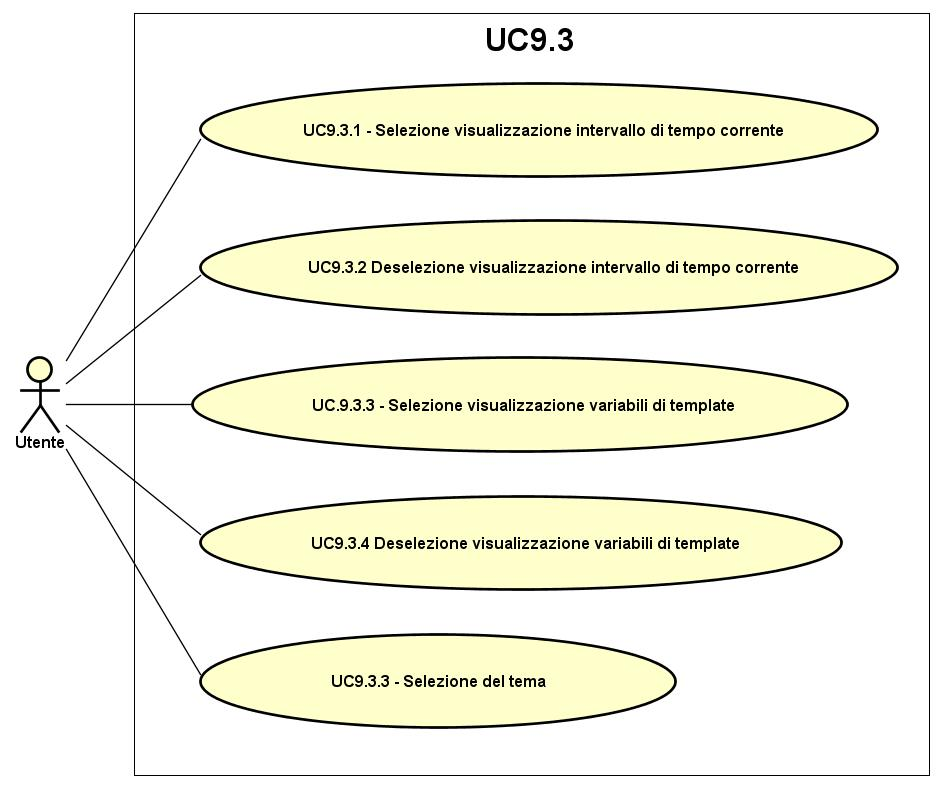
\includegraphics[scale=0.45]{Img/UC9-3}
	\caption{UC9.3: Selezione opzioni di visualizzazione}\label{}
\end{figure}
\begin{itemize}
	\item \textbf{Attori}: Utente;
	\item \textbf{Descrizione}: L'attore seleziona le opzioni per la visualizzazione dello snapshot della dashboard o di un panel;
	\item \textbf{Precondizione}: Il sistema permette la selezione di opzioni per la visualizzazione di snapshot;
	\item \textbf{Flusso principale degli eventi}:
	\begin{itemize}
		\item Selezione visualizzazione intervallo di tempo corrente (UC9.3.1);
		\item Deselezione visualizzazione intervallo di tempo corrente (UC9.3.2);
		\item Selezione visualizzazione variabili di template (9.3.3);
		\item Deselezione visualizzazione variabili di template (9.3.4);
		\item Selezione del tema (UC9.3.5).
	\end{itemize}
	\item \textbf{Postcondizione}: Le opzioni di visualizzazione dello snapshot sono state selezionate.
\end{itemize}

\subsection{UC9.3.1: Selezione visualizzazione intervallo di tempo corrente}
\begin{itemize}
	\item \textbf{Attori}: Utente;
	\item \textbf{Descrizione}: L'attore seleziona la visualizzazione dell'intervallo di tempo in cui sono stati raccolti i dati presenti nello snapshot;
	\item \textbf{Precondizione}: Il sistema permettere di selezionare la visualizzazione dell'intervallo di tempo in uno snapshot;
	\item \textbf{Postcondizione}: L'intervallo di tempo in cui sono stati raccolti i dati presenti viene visualizzato nello snapshot.
\end{itemize}

\subsection{UC9.3.2: Deselezione visualizzazione intervallo di tempo corrente}
\begin{itemize}
	\item \textbf{Attori}: Utente;
	\item \textbf{Descrizione}: L'attore deseleziona la visualizzazione dell'intervallo di tempo in cui sono stati raccolti i dati presenti nello snapshot;
	\item \textbf{Precondizione}: Il sistema permettere di deselezionare la visualizzazione dell'intervallo di tempo in uno snapshot;
	\item \textbf{Postcondizione}: L'intervallo di tempo in cui sono stati raccolti i dati presenti non viene visualizzato nello snapshot.
\end{itemize}

\subsection{UC9.3.3: Selezione visualizzazione variabili di template}
\begin{itemize}
	\item \textbf{Attori}: Utente;
	\item \textbf{Descrizione}: L'attore seleziona la visualizzazione delle variabili di template nello snapshot;
	\item \textbf{Precondizione}: Il sistema permette di selezionare la visualizzazione delle variabili di template in uno snapshot;
	\item \textbf{Postcondizione}: Le variabili di template vengono visualizzate nello snapshot.
\end{itemize}

\subsection{UC9.3.4: Deselezione visualizzazione variabili di template}
\begin{itemize}
	\item \textbf{Attori}: Utente;
	\item \textbf{Descrizione}: L'attore deseleziona la visualizzazione delle variabili di template nello snapshot;
	\item \textbf{Precondizione}: Il sistema permette di deselezionare la visualizzazione delle variabili di template in uno snapshot;
	\item \textbf{Postcondizione}: Le variabili di template no vengono visualizzate nello snapshot.
\end{itemize}

\subsection{UC9.3.5: Selezione del tema}
\begin{itemize}
	\item \textbf{Attori}: Utente;
	\item \textbf{Descrizione}: L'attore seleziona i colori di sfondo dello snapshot; 
	\item \textbf{Precondizione}: Il sistema permette la selezione di temi tra quelli predefiniti;
	\item \textbf{Postcondizione}: Il tema dello snapshot viene selezionato.
\end{itemize}
